\documentclass[a4paper,12pt]{article}
\usepackage[spanish]{babel}
\usepackage[utf8]{inputenc}
\usepackage{graphicx}
\usepackage{booktabs}
\usepackage{geometry}
\geometry{margin=2.5cm}
\title{Informe de Análisis de Datos de Salud Mental}
\author{Equipo Malackathon}
\date{\today}

\begin{document}
\maketitle

\section{Análisis descriptivo inicial}
\subsection{Dimensiones y estructura}
El dataset contiene \textbf{21,210 filas} y \textbf{111 columnas}.

\subsection{Tipos de variables}
\begin{itemize}
  \item \textbf{Fechas}: Fecha de nacimiento, Fecha de Ingreso, Fecha de Fin Contacto, etc.
  \item \textbf{Carácter/Textos}: Nombre, Diagnóstico Principal, Servicio, Centro Recodificado, etc.
  \item \textbf{Categóricas}: Comunidad Autónoma, Categoría, Procedimiento 9-20, POA Diagnóstico 1-20, etc.
  \item \textbf{Numéricas}: Sexo, Edad, Edad en Ingreso, Estancia Días, Reingreso, Coste APR, etc.
\end{itemize}

\subsection{Valores nulos o desconocidos}
Algunas columnas presentan valores nulos en todos los registros (ejemplo: CCAA Residencia, Procedimiento Externo 6). Otras columnas clave no presentan nulos (ejemplo: Comunidad Autónoma, Nombre, Fecha de nacimiento, Sexo, Edad en Ingreso).

\subsection{Estadísticos básicos}
\begin{tabular}{lcccc}
\toprule
Variable & Media & Mínimo & Máximo & Desviación estándar \\
\midrule
Edad en Ingreso & 43.7 & 0 & 96 & 14.1 \\
Sexo & 1.45 & 1 & 9 & 0.56 \\
\bottomrule
\end{tabular}

\subsection{Outliers}
Variables con outliers detectados (IQR):
\begin{itemize}
  \item Estancia Días: 1,229 posibles outliers
  \item Edad en Ingreso: 149 posibles outliers
  \item Otros: Coste APR, Riesgo Mortalidad APR, etc.
\end{itemize}

\subsection{Gráficas}
\begin{figure}[h!]
  \centering
  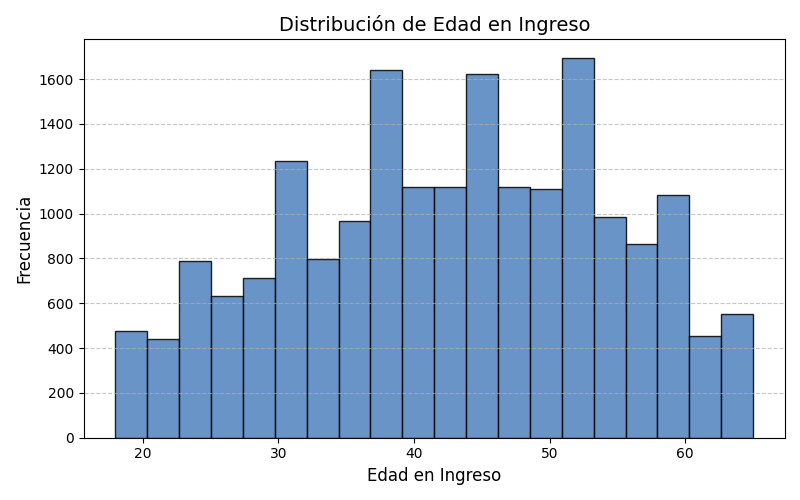
\includegraphics[width=0.7\textwidth]{hist_edad.png}
  \caption{Distribución de Edad en Ingreso}
\end{figure}

\begin{figure}[h!]
  \centering
  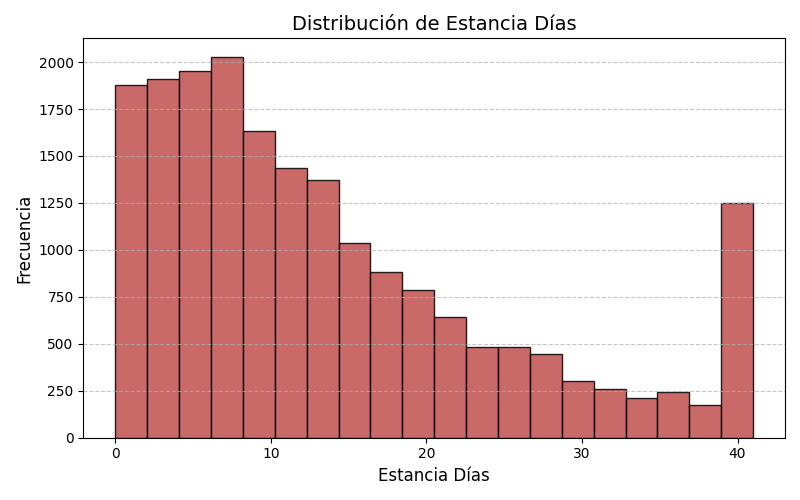
\includegraphics[width=0.7\textwidth]{hist_estancia.png}
  \caption{Distribución de Estancia Días}
\end{figure}

\newpage
\section{Ingeniería de características}
\subsection{Creación de nuevas variables}
\begin{itemize}
  \item \textbf{Edad agrupada}: Agrupar Edad en Ingreso en rangos (ejemplo: 0-18, 19-30, 31-50, 51+)
  \item \textbf{Año de ingreso}: Extraer el año de la columna Fecha de Ingreso
  \item \textbf{Duración estancia categorizada}: Categorizar Estancia Días (ejemplo: corta, media, larga)
\end{itemize}

\subsection{Transformaciones}
\begin{itemize}
  \item \textbf{Normalización y centrado}: Aplicar Z-score a Edad en Ingreso y Estancia Días
  \item \textbf{Winsorización}: Limitar valores extremos en variables continuas
\end{itemize}

\subsection{Codificación}
\begin{itemize}
  \item \textbf{Sexo binario}: 1=Hombre, 2=Mujer $\rightarrow$ 0/1
  \item \textbf{One-hot encoding}: Para Comunidad Autónoma, Categoría, etc.
\end{itemize}

\vspace{1cm}
\noindent Este informe resume el análisis inicial y las propuestas de ingeniería de variables para el dataset de salud mental. Para detalles completos, consultar el archivo \texttt{analisis\_salud\_mental.txt} y los scripts de procesamiento.

\end{document}
